\documentclass{beamer}
\usepackage[utf8]{inputenc}
\usepackage[english]{babel}
\usepackage{helvet}
\usepackage[T1]{fontenc}
\usepackage[inline]{asymptote}
\usepackage{asy_helper}
\usepackage{slide_helper}
\usepackage{cancel}
\usepackage{tikz}
\usetikzlibrary{shapes.geometric, arrows}
\usepackage{pgfplots}
\pgfplotsset{compat=1.5} 
\usepgfplotslibrary{statistics}
\usetikzlibrary{external}
\tikzexternalize%

\title[MA205 - Section 4.3]{Binomial Distribution}

\newcommand{\prob}[1]{P\left({#1}\right)}
\newcommand{\jointprob}[3]{\prob{{#1}~\text{#2}~{#3}}}
\newcommand{\condprob}[2]{\prob{{#1}~|~{#2}}}
\newcommand{\comb}[2]{_{#1}C_{#2}}

\newcommand<>{\success}[1]{{\color#2{green!70!black}#1}}
\newcommand<>{\failure}[1]{{\color#2{red!80}#1}}

\begin{document}
\begin{frame}
\titlepage
\end{frame}

\begin{frame}
  \begin{example}\label{twitter}
    \vspace{-2mm} % beamer bug
    Let us assume there is a 0.85 probability that a randomly chosen adult has heard of Twitter.\pause

    \vspace{1mm}
    Four people are chosen at random:

    \vspace{-2.5mm}
    \begin{center}
    Ariana ($A$), \quad
    Brittany ($B$), \quad
    Carlton ($C$), \quad
    Damian ($D$)
    \end{center}

    \vspace{-2mm}
    We want the probability exactly one of them will have heard of Twitter.\pause

    \vspace{1mm}
    There are four combinations possible:

    \vspace{-7mm}
    \begin{equation*}
      \begin{array}{l}
        \prob{A = \success<3-5>{\text{yes}}~\text{and}~
              B = \failure<3-5>{\text{no}}~\text{and}~
              C = \failure<3-5>{\text{no}}~\text{and}~
              D = \failure<3-5>{\text{no}}}\\
        \onslide<4->
        \qquad = \success<4-5>{0.85} \cdot \failure<4-5>{0.15}\cdot \failure<4-5>{0.15}\cdot \failure<4-5>{0.15}
        \onslide<5->
        = {(\success<5>{0.85})}^1{(\failure<5>{0.15})}^3 = 0.002869 \\
        \onslide<6->
        \prob{A = \failure<6-8>{\text{no}}~\text{and}~
              B = \success<6-8>{\text{yes}}~\text{and}~
              C = \failure<6-8>{\text{no}}~\text{and}~
              D = \failure<6-8>{\text{no}}}\\
        \onslide<7->
        \qquad = \failure<7-8>{0.15} \cdot \success<7-8>{0.85}\cdot \failure<7-8>{0.15}\cdot \failure<7-8>{0.15}
        \onslide<8->
        = {(\success<8>{0.85})}^1{(\failure<8>{0.15})}^3 = 0.002869 \\
        \onslide<9->
        \prob{A = \failure<9-11>{\text{no}}~\text{and}~
              B = \failure<9-11>{\text{no}}~\text{and}~
              C = \success<9-11>{\text{yes}}~\text{and}~
              D = \failure<9-11>{\text{no}}}\\
        \onslide<10->
        \qquad = \failure<10-11>{0.15} \cdot \failure<10-11>{0.15}\cdot \success<10-11>{0.85}\cdot \failure<10-11>{0.15}
        \onslide<11->
        = {(\success<11>{0.85})}^1{(\failure<11>{0.15})}^3 = 0.002869 \\
        \onslide<12->
        \prob{A = \failure<12-14>{\text{no}}~\text{and}~
              B = \failure<12-14>{\text{no}}~\text{and}~
              C = \failure<12-14>{\text{no}}~\text{and}~
              D = \success<12-14>{\text{yes}}}\\
        \onslide<13->
        \qquad = \failure<13-14>{0.15} \cdot \failure<13-14>{0.15}\cdot \failure<13-14>{0.15}\cdot \success<13-14>{0.85}
        \onslide<14->
        = {(\success<14>{0.85})}^1{(\failure<14>{0.15})}^3 = 0.002869 \\
      \end{array}
    \end{equation*}

    \vspace{-3mm}
    \onslide<15->
    So, the probability exactly one has heard of Twitter is
    \vspace{-4mm}
    \begin{equation*}
      0.002869 + 0.002869 + 0.002869 + 0.002869 = 0.11475 = 11.475\%
    \end{equation*}
  \end{example}
\end{frame}

\begin{frame}
  \begin{definition}
    The \textbf{binomial distribution} is used to describe the number of successes in a fixed number or trials.
  \end{definition}\pause

  \begin{block}{Notation}
    \begin{center}
      \begin{tabular}{ll}
        $p$ & The probability of a success. \\
        $q = 1-p$ & The probability of a failure. \\
        $n$ & The fixed number of trials. \\
        $k$ & The number of successes.
      \end{tabular}
    \end{center}
  \end{block}\pause

  \begin{note}
    Example~\ref{twitter} is how to find a binomial distribution the hard way.
  \end{note}\pause

  \begin{note}
    If all the scenarios are independent of each other, then we can calculate the final probability as:

    \vspace{-4mm}
    \begin{equation*}
      \begin{aligned}
        \left[\text{\# of scenarios}\right] \cdot \prob{\text{single scenario}}
      \end{aligned}
    \end{equation*}
  \end{note}
\end{frame}

\begin{frame}
  \begin{definition}
    The \textbf{factorial}, for any positive integer $n$, is

    \vspace{-3mm}
    \begin{equation*}
      \begin{aligned}
        0! &= 1 \\
        1! &= 1 \\
        2! &= 2\cdot 1 = 2 \\
        3! &= 3\cdot 2\cdot 1 = 6 \\
        4! &= 4\cdot 3\cdot 2\cdot 1 = 24 \\
        &\vdots \\
        n! &= n\cdot(n-1) \cdot(n-2)\cdot \cdots \cdot 4\cdot 3\cdot 2\cdot 1
      \end{aligned}
    \end{equation*}
  \end{definition}\pause

  \begin{note}
    Factorials can be calculated iteratively.\ i.e.\@
    \begin{equation*}
      \begin{aligned}
        (n+1)! &= n!\cdot (n+1)
      \end{aligned}
    \end{equation*}
  \end{note}
\end{frame}

\begin{frame}
  \begin{definition}
    The \textbf{binomial coefficients} gives the number of ways to choose $k$ successes in $n$ trials.:
    \begin{equation*}
      \begin{aligned}
        \binom{n}{k} = \dfrac{n!}{k!(n-k)!}
      \end{aligned}
    \end{equation*}
    Read \textquote{$n$ choose $k$.}
  \end{definition}\pause

  \begin{example}
    The number of ways to choose $k=3$ successes in $n=4$ trials:
    \begin{equation*}
      \begin{aligned}
        \binom{4}{3} \pause
        = \dfrac{4!}{3!(4-3)!} \pause
        = \dfrac{4!}{3!1!} \pause
        = \dfrac{4\cdot 3\cdot 2\cdot 1}{3\cdot 2\cdot 1\cdot 1} \pause
        = \dfrac{4\cdot \cancel{3}\cdot \cancel{2}\cdot 1}{\cancel{3}\cdot \cancel{2}\cdot 1\cdot 1} \pause
        = 4
      \end{aligned}
    \end{equation*}
  \end{example}
\end{frame}

\begin{frame}
  \begin{block}{Binomial Distribution}
    Suppose the probability of a single trial being a success is $p$. Then the probability of observing exactly $k$ successes in $n$ independent trials is given by
    \begin{equation*}
      \begin{aligned}
        \binom{n}{k}p^k{(1-p)}^{n-k} = \dfrac{n!}{k!(n-k)!} p^k {(1-p)}^{n-k}
      \end{aligned}
    \end{equation*}
    The mean, variance, and standard deviation of the number of observed successes are
    \begin{equation*}
      \mu = np, \qquad
      \sigma^2 = np(1-p), \qquad
      \sigma = \sqrt{np(1-p)}
    \end{equation*}
  \end{block}\pause
  
  \begin{block}{Is It Binomial?}
    Every binomial distribution has to satisfy the following:
    \begin{itemize}
    \item The trials are independent.\pause
    \item The number of trials, $n$, is fixed.\pause
    \item Each trial outcome can be classified as either a \emph{success} or \emph{failure}.\pause
    \item The probability of a success, $p$, is the same for each trial.
    \end{itemize}
  \end{block}
\end{frame}

\begin{frame}
  \begin{example}
    From Example~\ref{twitter} we have $p=0.85$, $n=4$, and $k=1$.\pause

    \vspace{-6mm}
    \begin{equation*}
      \begin{aligned}
        \prob{\text{exactly one has heard of twitter}}
        &= \binom{n}{k}p^k{(1-p)}^{n-k} \\\pause
        &= \binom{4}{1}{(0.85)}^{1}{(1-0.85)}^{4-1} \\\pause
        &= \dfrac{4!}{1!(4-1)!} {(0.85)}^{1} {(0.15)}^{3} \\\pause
        &= \dfrac{4 \cdot 3\cdot 2\cdot 1}{1\cdot 3\cdot 2\cdot 1} {(0.85)}^{1} {(0.15)}^{3} \\\pause
        &= \dfrac{4 \cdot \cancel{3}\cdot \cancel{2}\cdot 1}{1\cdot \cancel{3}\cdot \cancel{2}\cdot 1} {(0.85)}^{1} {(0.15)}^{3} \\\pause
        &= 4\cdot {(0.85)}^{1} {(0.15)}^{3} \\\pause
        &= 0.11475
      \end{aligned}
    \end{equation*}
  \end{example}
\end{frame}

\begin{frame}
  \begin{example}
    Assume that 70\% of customers won't exceed their car insurance deductible. Let's the probability that 5 of 8 randomly selected customers won't exceed their premium.\pause

    \vspace{1mm}
    Start by identifying

    \vspace{-3.5mm}
    \begin{equation*}
      \begin{aligned}
        p=0.7, \qquad
        q=1-p=0.3, \qquad
        n=8, \qquad
        k=5
      \end{aligned}
    \end{equation*}\pause

    \vspace{-11mm}
    \begin{equation*}
      \begin{aligned}
        \binom{n}{k}p^k{(1-p)}^{n-k}
        &= \binom{8}{5}{(0.7)}^{5}{(0.3)}^{8-5} \\\pause
        &= \dfrac{8!}{5!(8-5)!} {(0.7)}^{5}{(0.3)}^{3}\pause
        = \dfrac{8!}{5!(3)!} {(0.7)}^{5}{(0.3)}^{3} \\\pause
        &= \dfrac{8\cdot 7\cdot 6\cdot 5\cdot 4\cdot 3\cdot 2\cdot 1}{5\cdot 4\cdot 3\cdot 2\cdot 1\cdot 3\cdot 2\cdot 1} {(0.7)}^{5}{(0.3)}^{3} \\\pause
        &= \dfrac{8\cdot 7\cdot 6\cdot \cancel{5}\cdot \cancel{4}\cdot \cancel{3}\cdot \cancel{2}\cdot 1}{\cancel{5}\cdot \cancel{4}\cdot \cancel{3}\cdot \cancel{2}\cdot 1\cdot 3\cdot 2\cdot 1} {(0.7)}^{5}{(0.3)}^{3} \\\pause
        &= 56\cdot {(0.7)}^{5}{(0.3)}^{3} \\\pause
        &= 0.254122
      \end{aligned}
    \end{equation*}
  \end{example}
\end{frame}

\begin{frame}
  \begin{example}
    Assume the probability that a smoker will develop a severe lung condition in their life time is 0.3.

    \vspace{1mm}
    \question{If you have four friends who smoke, are the conditions for the binomial model satisfied?}\pause
    \answer{It is likely that independence is not satisfied, since they probably all know each other.}
  \end{example}\pause

  \begin{example}
    Suppose instead four people are randomly selected.

    \vspace{1mm}
    \question{Is the binomial model appropriate to find the probability that none of them will develop a severe lung condition?}
    \answer{We are assuming that the four are randomly selected, yes.

      \vspace{-5mm}
      \begin{equation*}
        \begin{aligned}
          \binom{n}{k}p^k{(1-p)}^{n-k}
          &= \binom{4}{0}{(0.3)}^0{(1-0.3)}^{4-0}
          = \dfrac{4!}{0!(4-0)!} {(0.3)}^0 {(0.7)}^{4} \\
          &= 1\cdot 1\cdot {(0.7)}^{4}
          = 0.2401
        \end{aligned}
      \end{equation*}
    }
    \vspace{-4mm}
  \end{example}
\end{frame}

\begin{frame}
  \begin{example}\label{smokers}
    \vspace{-2mm} % beamer bug
    Let consider finding the probability than no more than one of the four people will develop a severe lung condition.\pause

    \vspace{1mm}
    The events that \textquote{none of them develops a severe lung condition} and \textquote{exactly one develops a severe lung condition} are mutually exclusive.

      \vspace{-5mm}
      \begin{equation*}
        \begin{aligned}
          \prob{\text{none}} &+ \prob{\text{exactly one}} \\\pause
          & = \binom{4}{0}{(0.3)}^0{(1-0.3)}^{4-0} + \binom{4}{1}{(0.3)}^1{(1-0.3)}^{4-1} \\\pause
          &= \dfrac{4!}{0!(4-0)!} {(0.3)}^0 {(0.7)}^{4} + \dfrac{4!}{1!(4-1)!} {(0.3)}^1 {(0.7)}^{3} \\\pause
          &= \dfrac{4\cdot 3\cdot 2\cdot 1}{1\cdot 4\cdot 3\cdot 2\cdot 1} {(0.3)}^0 {(0.7)}^{4} + \dfrac{4\cdot 3\cdot 2\cdot 1}{1\cdot 3\cdot 2\cdot 1}  {(0.3)}^1 {(0.7)}^{3} \\\pause
          &= \dfrac{\cancel{4}\cdot \cancel{3}\cdot \cancel{2}\cdot 1}{1\cdot \cancel{4}\cdot \cancel{3}\cdot \cancel{2}\cdot 1} {(0.3)}^0 {(0.7)}^{4} + \dfrac{4\cdot \cancel{3}\cdot \cancel{2}\cdot 1}{1\cdot \cancel{3}\cdot \cancel{2}\cdot 1}  {(0.3)}^1 {(0.7)}^{3} \\\pause
          &= 0.2401 + 0.4116 \\\pause
          &= 0.6517 = 65.17\%
        \end{aligned}
      \end{equation*}
  \end{example}
\end{frame}

\begin{frame}
  \begin{example}
    Lets consider finding the probability that at least two of the four people will develop a severe lung condition.\pause

    \vspace{1mm}
    The complement of \textquote{at least two will develop a severe lung condition} is \textquote{no more than one will develop a severe lung condition.}\pause

    \vspace{1mm}
    We know from Example~\ref{smokers} that $\prob{\text{no more than one}} = 0.6517$.\pause

    \vspace{1.5mm}
    So,

    \vspace{-6mm}
    \begin{equation*}
      \begin{aligned}
        \prob{\text{at least two}}
        &= 1 - \prob{\text{no more than one}} \\\pause
        &= 1 - 0.6517 \pause
        = 0.3483 = 34.83\%
      \end{aligned}
    \end{equation*}
  \end{example}\pause

  \begin{example}
    \question{Out of seven randomly selected smokers, how many would we expect to develop a severe lung condition?}\pause
    \answer{The mean of the binomial model is

      \vspace{-4.3mm}
      \begin{equation*}
        \begin{aligned}
          \mu &= np \pause
          = 7\cdot 0.3 \pause
          = 2.1
        \end{aligned}
      \end{equation*}

      \vspace{-2mm}
      On average, we would expect 2.1 of 7 randomly chosen smokers to develop a severe lung condition.
      }
  \end{example}
\end{frame}

\begin{frame}
  \begin{example}
    \begin{equation*}
      \begin{aligned}
        \binom{n}{0}\pause
        &= \dfrac{n!}{0!(n-0)!}\pause
        = \dfrac{n!}{n!}\pause
        = 1\pause
      \end{aligned}
    \end{equation*}
  \end{example}

  \begin{example}
    \begin{equation*}
      \begin{aligned}
        \binom{n}{1}\pause
        &= \dfrac{n!}{1!(n-1)!}\pause
        = \dfrac{n!}{(n-1)!}\pause
        = \dfrac{n\cdot(n-1)!}{(n-1)!}\pause
        = n\pause
      \end{aligned}
    \end{equation*}
    \end{example}

    \begin{example}
    \begin{equation*}
      \begin{aligned}
        \binom{n}{n-1}\pause
        &= \dfrac{n!}{(n-1)!(n-(n-1))!}\pause
        = \dfrac{n!}{(n-1)!1!}\pause
        = \dfrac{n\cdot(n-1)!}{(n-1)!}\pause
        = n\pause
      \end{aligned}
    \end{equation*}
      \end{example}

      \begin{example}
    \begin{equation*}
      \begin{aligned}
        \binom{n}{n}\pause
        &= \dfrac{n!}{n!(n-n)!}\pause
        = \dfrac{n!}{n!0!}\pause
        = \dfrac{n!}{n!}\pause
        = 1
      \end{aligned}
    \end{equation*}
  \end{example}
\end{frame}

\begin{frame}
  \begin{example}\label{less smokers}
    \vspace{-2mm}
    Approximately 15\% of the US population smokes cigarettes.\pause

    \vspace{1mm}
    A local government believed their community has a lower smoker rate and commissioned a survey of 400 randomly selected individuals.\pause

    \vspace{1mm}
    The survey found that only 42 of the 400 participants smoke cigarettes.\pause

    \vspace{1mm}
    If the true proportion of smokers in the community was really 15\%, what is the probability of observing 42 or fewer smokers in a sample of 400 people?\pause

    \vspace{-2mm}
    \begin{equation*}
      \begin{aligned}
        &\prob{k=0~\text{or}~k=1~\text{or}~\cdots~\text{or}~k=42}\\\pause
        &\quad = \prob{k=0}+\prob{k=1}+\cdots+\prob{k=42} \\\pause
        &\quad = 5.8558\times10^{-29} + 4.133335\times10^{-27}+\cdots+0.001985 \\\pause
        &\quad = 0.0054
      \end{aligned}
    \end{equation*}
  \end{example}\pause

  \begin{note}
    When certain conditions are met, we can actually use the normal distribution to approximate the binomial distribution.
  \end{note}
\end{frame}

\begin{frame}
  \begin{example}
    \begin{center}
      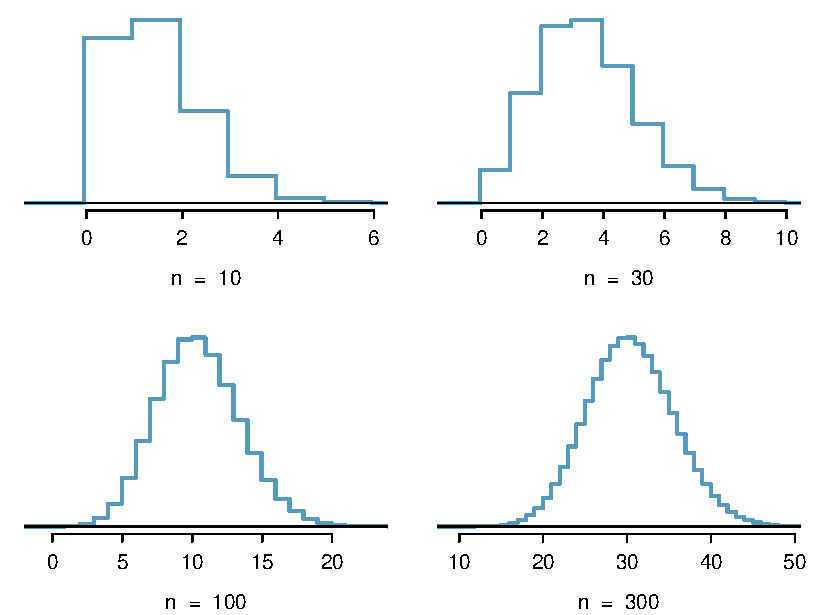
\includegraphics[scale=0.7]{fourBinomialModelsShowingApproxToNormal.pdf}

      \vspace{0mm}
      Histograms of samples from the binomial model when $p=0.10$.
    \end{center}
  \end{example}
\end{frame}

\begin{frame}
  \begin{block}{Normal Approximation of the Binomial Distribution}
    The binomial distribution with probability of success $p$ is approximately normal when the sample size $n$ is sufficiently large so that:
    \begin{equation*}
      \begin{aligned}
        np \geq 10
        \qquad\text{and}\qquad
        n(1-p) \geq 10
      \end{aligned}
    \end{equation*}

    \vspace{1mm}
    The approximate normal distribution has parameters corresponding to the mean and standard deviation of the binomial distribution:
    \begin{equation*}
      \begin{aligned}
        \mu=np
        \qquad\qquad\qquad
        \sigma=\sqrt{np(1-p)}
      \end{aligned}
    \end{equation*}
  \end{block}
\end{frame}

\begin{frame}
  \begin{example}
    Let us check to see if the binomial distribution in Example~\ref{less smokers} is approximately normal.\pause

    \vspace{1mm}
    Recall that $p=0.15$, $n=400$, so we check:

    \vspace{-3mm}
    \begin{equation*}
      \begin{aligned}
        np &=\pause 400\cdot0.15\pause = 60\pause \geq 10 \\\pause
        n(1-p) &=\pause 400\cdot(1-0.15)\pause = 400\cdot0.85\pause = 340\pause \geq 10
      \end{aligned}
    \end{equation*}\pause

    \vspace{-3mm}
    We may now use the normal distribution to approximate the binomial distribution for observing 42 or fewer smokers:

    \vspace{-3mm}
    \begin{equation*}
      \begin{aligned}
        \mu &= np\pause = 60 \\\pause
        \sigma &= \sqrt{np(1-p)}\pause = 7.14143 \\\pause
        z &= \dfrac{x-\mu}{\sigma}\pause = \dfrac{42-60}{7.14143}\pause = -2.5205
      \end{aligned}
    \end{equation*}\pause

    \vspace{-3mm}
    Using technology gives:

    \vspace{-4mm}
    \begin{equation*}
      \begin{aligned}
        \prob{z\leq -2.52} = 0.005859
      \end{aligned}
    \end{equation*}

    \vspace{-2mm}
    This is very close to the value of 0.0054 we calculated in Example~\ref{less smokers}.
  \end{example}
\end{frame}

\begin{frame}
  \begin{example}
    Suppose we want to compute the probability of observing 49, 50, or 51 smokers in 400 when $p=0.15$.\pause

    \vspace{1mm}
    It's tempting to apply the normal approximation here, as well. But,

    \vspace{-3mm}
    \begin{equation*}
      \begin{aligned}
        \text{Binomial:}~0.0649
        \qquad\qquad
        \text{Normal:}~0.0421
      \end{aligned}
    \end{equation*}\pause

    \vspace{-6mm}
    \begin{center}
      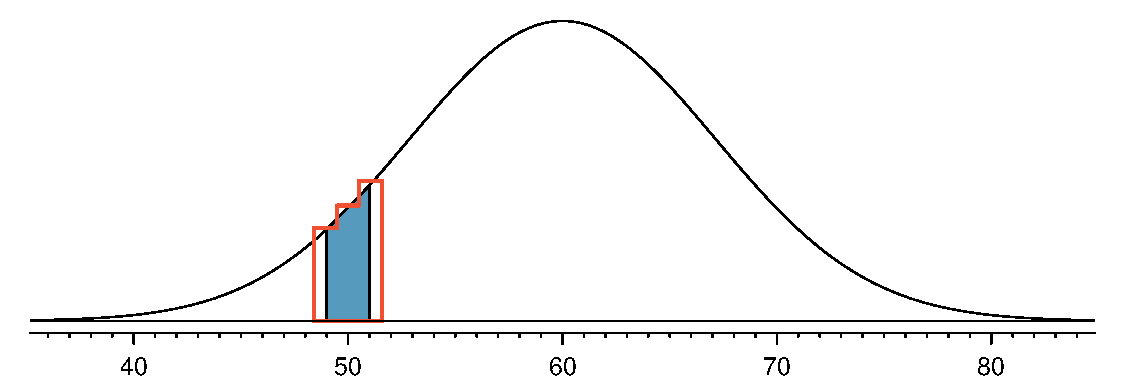
\includegraphics[scale=0.6]{normApproxToBinomFail.pdf}
    \end{center}

    \vspace{-2mm}
    The area representing the binomial probability is outlined in red while the area representing the normal approximation is shaded in blue. Notice that the width of the normal approximation is too narrow.
    
  \end{example}
\end{frame}

\begin{frame}
  \begin{block}{Improving the Normal Approximation}
    The normal approximation to the binomial distribution for intervals of values is usually improved if the cutoff values are modified slightly.

    \vspace{1mm}
    The cutoff values for the lower end of a shaded region should be reduced by 0.5.

    \vspace{1mm}
    The cutoff values for the upper end of a shaded region should be increased by 0.5.
  \end{block}\pause

  \begin{example}
    For computing the probability of observing 49, 50, or 51 smokers in 400 when $p=0.15$ we get the three values:
    \begin{equation*}
      \begin{aligned}
        \text{Binomial:}&~0.0649 \\
        \text{Unmodified Normal:}&~0.0421 \\
        \text{Modified Normal:}&~0.0633
      \end{aligned}
    \end{equation*}
  \end{example}
\end{frame}
\end{document}
